\section{Auswertung}
\label{sec:Auswertung}

\subsection{Messdaten und Diagramm}
Die Messwerte sind in einer Tabelle aufgetragen. Dabei sind die Temperaturen einmal in $\si{\celsius}$ und einmal in $\si{\kelvin}$ angegeben, 
den Drücken ist nach Anleitung \cite{anleitung} ein bar dazuaddiert worden.
\begin{table}
  \begin{tabular}{
    S[table-format=2.1] %Zeit
    S[table-format=2.1] %tempc
    S[table-format=3.2] %tempK
    S[table-format=2.2] %p_1
    S[table-format=2.1] %tempC
    S[table-format=3.2] %tempK
    S[table-format=1.1] %p_2
    S[table-format=3.0] %N
  }
  \toprule
  {$ t \mathbin{/} \si{\minute} $} &
  {$ T_1 \mathbin{/} \si{\celsius} $} &
  {$ T_2 \mathbin{/} \si{\kelvin}$} &
  {$ p_1 \mathbin{/} \si{\bar}$} &
  {$ T_2 \mathbin{/} \si{\celsius}$} &
  {$ T_2 \mathbin{/} \si{\kelvin}$} &
  {$ p_2 \mathbin{/} \si{\bar}$} &
  {$N_{\text{mech}} \mathbin{/} \si{\watt}$} \\
  \midrule
  \input{hope.txt}
  \end{tabular}
\end{table}

Dann haben wir die Temperaturen in $\si{\kelvin}$ gegen die Zeit in einem Diagramm aufgetragen. 
Die Verläufe haben wir mit einem Polynom 2. Grades ($T(t) = a\cdot t² + b\cdot t + c$)angenähert.
\begin{figure}
  \centering
  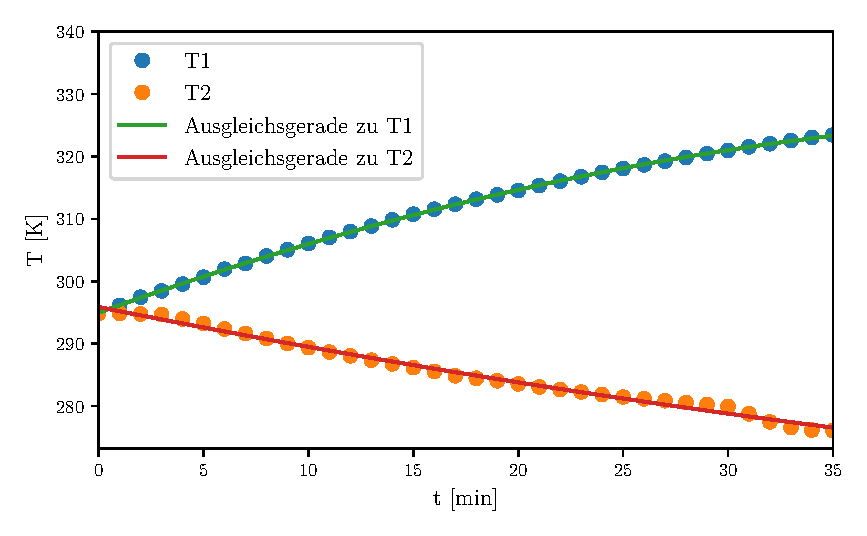
\includegraphics{tempK.pdf}
  \caption{Die gemessenen Temperaturen in Zeitverlauf mit den angenäherten Funktionen.}
  \label{fig:tempK}
\end{figure}
Für die Ausgleichsrechnung ergeben sich für die Konstanten $a, b$ und $c$:
\begin{align*}
  \intertext{Für } T_1(t)&=T(t):& \intertext{Für } T_2(t) &= T(t):\\
  a&=\SI{-0.0116}{\kelvin\per\second\squared}  & a&= \SI{0.0034}{\kelvin\per\second\squared}\\
  b&=\SI{1.2168}{\kelvin\per\second} & b&=\SI{-0.6725}{\kelvin\per\second} \\
  c&=\SI{294.9701}{\kelvin} & c&=\SI{295.8702}{\kelvin} \\
  \implies T_1(t) &= -0.0116t²+1.2168t+294.9701 &\implies T_2(t) &= 0.0034t² -0.6725t + 295.8702
\end{align*}

\subsection{Bestimmung der Güteziffer}
Zur Bestimmung der Güteziffer errechnen wir die Differantialquotienten $\frac{\symup{d}T_1}{\symup{d}t}$ und $\frac{\symup{d}T_2}{\symup{d}t}$ für vier verschiedene Zeitpunkte:
Die Ableitung ist aus der Ausgleichsrechnung einfach bestimmt.
\begin{equation}
  \frac{\symup{d}T}{\symup{d}t} = 2at + b
\end{equation}
Für $T_1$ ergeben sich die Ableitungen zu:
\begin{gather*}
  \text{bei} t=1.0 : \frac{\symup{d}T_1}{\symup{d}t} = \SI{1.1936}{\kelvin\per\second}\\  %Fehler von Gaus
  \text{bei} t=2.0 : \frac{\symup{d}T_1}{\symup{d}t} = \SI{1.1704}{\kelvin\per\second}\\
  \text{bei} t=3.0 : \frac{\symup{d}T_1}{\symup{d}t} = \SI{1.1471}{\kelvin\per\second}\\
  \text{bei} t=4.0 : \frac{\symup{d}T_1}{\symup{d}t} = \SI{1.1239}{\kelvin\per\second}
\end{gather*}
Für $T_2$ ergeben sich die Ableitungen zu:
\begin{gather*}
  \text{bei} t=1.0 : \frac{\symup{d}T_2}{\symup{d}t} = \SI{-0.6656}{\kelvin\per\second}\\
  \text{bei} t=2.0 : \frac{\symup{d}T_2}{\symup{d}t} = \SI{-0.6588}{\kelvin\per\second}\\
  \text{bei} t=3.0 : \frac{\symup{d}T_2}{\symup{d}t} = \SI{-0.6519}{\kelvin\per\second}\\
  \text{bei} t=4.0 : \frac{\symup{d}T_2}{\symup{d}t} = \SI{-0.6450}{\kelvin\per\second}
\end{gather*}

Mit den Formel \refeq{eqn:gueteziffer} und \refeq{eqn:idguete} lassen sich nun die Güteziffer und die ideale Güteziffer berechnen.
Die Wärmekapazität der Kupferschlangen und des Wasser ergeben sich zu:
\begin{align*}
  m_kc_k &= \SI{750}{\joule\per\kelvin}\\
  mc_w &= 4 \cdot \SI{4184}{\joule\per\kelvin\kilo\gram} = \SI{16736}{\joule\per\kelvin} %muss ich citen ?
\end{align*}

\begin{table}
  \caption{Bestimmung der Güteziffer aus der Messreihe $T_1$}
  \begin{tabular}{
    S[table-format=3.0] %Zeit
    S[table-format=3.4] %guete gerechnet
    @{${}\pm {}$}
    S[table-format=3.2] %fehler der gueteziffer 
    S[table-format=3.4] %guete ideal
    S[table-format=2.2] %Abweichung
  }
  \toprule
  {$ t \mathbin{/} \si{\second} $} &
  \multicolumn{2}{c}{$ \nu $}&
  {$ \nu_{\text{id}}$} &
  {$ \text{Abweichung} \mathbin{/} \si{\percent}$} \\
  \midrule
  60&   173.9232& 95.7291  & 227.8077 &23.65\\
  120&  170.5397& 96.1649  & 110.1667   &54.80\\
  180&  167.1562& 96.8867  & 78.5395    &112.83\\
  240&  163.7728& 97.8885  & 53.4911    &206.17\\
  \end{tabular}
\end{table}

Der Fehler $\Delta \nu$ wurde mit der Fehlerfortpflanzung von Gauss berechnet.
Man erkennt eine große Abweichung der errechneten Werte für die Güteziffer und den dazu passenden Werten der idealen Güteziffer $\nu_{\text{id}}$.
Dies folgt einerseits aus den Annahmen, es handle sich um einen reversiblen Prozess und der Kompressor arbeite adiabatisch, welche nicht der Realität entsprechen.
Zusätzlich haben wir Energieverluste aus Reibung nicht beachtet. 
In der Diskussion gehen wir nochmal weiter auf mögliche Fehlerquellen ein.

\subsection{Bestimmung des Massendurchsatzes}
Zur Berechnung des Massendurchsatzes benötigen wir die Verdampfungswärme $L$. 
Diese kann wie folgt aus den gemessenen Werte errechnet werden. 
Zuerst erstellt man ein $(p,T)$ Diagramm, wobei die Temperatur als $\frac{1}{T}$ und der Druck als $\log(\frac{p}{p_0})$ mit Umgebungsdruck $p_0$ aufgetragen werden.
Mithilfe einer Ausgleichgerade bestimmt man die Steigung $m$ und kann dann durch $L=-m\cdot R$ die Verdampfungswärme L errechnen. 
$R$ entspricht der allgemeinen Gaskonstante.

\begin{figure}
  \centering
  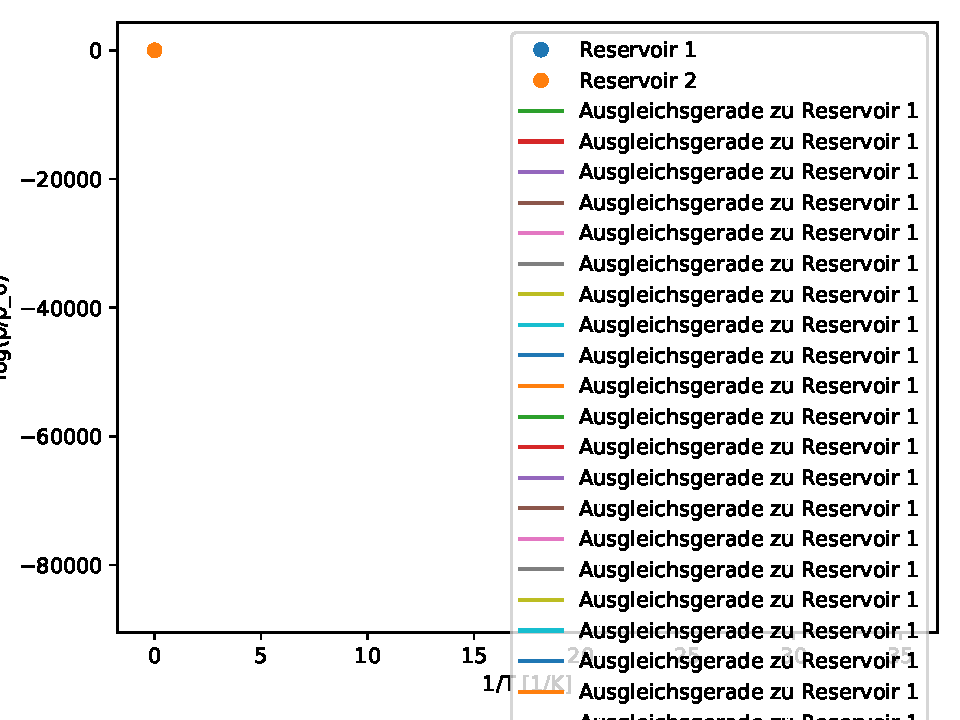
\includegraphics{TempDruck.pdf}
\end{figure}

Für die Ausgleichsgeraden für $\log(\frac{p}{p_0}) = m\cdot\frac{1}{T} + b$ ergeben sich:
\begin{align*}
  \text{für}T_1 \text{und} p_}\text{a}}: m&= \SI{-2462.4863 \pm 70.5436}{\kelvin} & b&=\num{8.5260 \pm 0.2268} \\
  \text{für}T_2 \text{und} p_{\text{b}}: m&= \SI{-1719.8296 \pm 88.3692}{\kelvin} & b&=\num{5.6974 \pm 0.3097}
\end{align*}
Da wir den Massendurchsatz aus den Messwerten bezüglich Reservoir 2 berechnen, werden wir zur Berechnung von $L$ auch die Steigung bezüglich Reservoir 2 benutzen.
Mit Fehlerrechnung nach \cite{fehler} erhalten wir für $L$ :
\begin{equation*}
  L = \SI{14298.6636\pm 734.6999}{\joule\per\mole}
\end{equation*}

Mit der bekannten Verdampfungswärme L lässt sich der Massendurchsatz zu unseren Differentialquotienten nach \eqref{eqn:massendurchsatz} berechnen.
\begin{table}
  \centering
  \begin{tabular}{S[table-format=3.0]
                  S[table-format=1.4]
                  S[table-format=1.4]}
    \toprule
    {$t \mathbin{/} \si{\second}$}&
    {$\frac{\symup{d}m}{\symup{d}t}\mathbin{/}\si{\mole\per\second}$}&
    {$\frac{\symup{d}m}{\symup{d}t}\mathbin{/}\si{\gram\per\second}$}\\
    \midrule
    60&   -0.00678  &  -0.8136    \\
    120&  -0.00671  &  -0.8052   \\
    180&  -0.00664  &  -0.7968    \\
    240&  -0.00657  &  -0.7884    \\
    \bottomrule    
  \end{tabular}
\end{table}

Für ein leichteres Weiterrechnen haben wir den Massendurchsatz zusätzlich noch in SI-Einheiten aufgeschrieben.
Dafür multipliziert man den Massendurchsatz mit der molaren Masse, die sich zu $M=\SI{120.9}{\gram\per\mole}$ ergibt.

\subsection{Bestimmung der mechanischen Kompressionsleistung $N_{\text{mech}}$}
Um die Formel \eqref{eqn:kompressorleistung} zur Berechung der mechanischen Kompressorleistung zu benutzen, 
müssen wir $\rho$ aus der idealen Gasgleichung mithilfe der angegebenen Werte errechnen.
Aus der Anleitung\cite[7]{anleitung} entnehmen wir $\rho_0 = \SI{5.51}{\gram\per\litre}$ bei $T=\SI{0}{\celsius}=\SI{273.25}{\kelvin}$ und $\kappa = \num{1.14}$, außerdem wissen wir $R=\SI{8.314}{\joule\per\mole\kelvin}$.
\begin{equation*}
  p\cdot V = n\cdot R\cdot T \implies nR = \frac{pV}{T}
\end{equation*}
Da die Stoffmenge über die Zeit konstant bleibt, folgt $nR=$const., außerdem ist $\rho \cdot V = m$.
\begin{gather*}
  \frac{p_0 V_0}{T_0} = \frac{p_{\text{a}} V_2}{T_2}\\
  \implies \frac{p_0m}{\rho_0 T_0} = \frac{p_{\text{a}} m}{\rho T_2}\\
  \implies \rho = \frac{\rho_0T_0 \cdot p_{\text{a}} }{p_0 \cdot T_2}
\end{gather*}

\begin{table}
  \caption{Mechanische Kompressorleistung zu verschiedenen Zeitpunkten.}
  \begin{tabular}{S[table-format=3.0]
                  S[table-format=3.2]}
    \toprule
    {$t \mathbin{/} \si{\second}$}&{$N_{\text{mech}} \mathbin{/} \si{\watt}$}\\
    \midrule
    60& 152.08\\
    120& 163.83 \\
    180&  182.19\\
    240& 179.84 \\
    \bottomrule    
  \end{tabular}
\end{table}